\documentclass[12pt,a4paper]{article}

% ─── Paquetes ───────────────────────────────────────────────────────────────
\usepackage[utf8]{inputenc}
\usepackage[T1]{fontenc}
\usepackage{amsmath,amssymb,amsthm}
\usepackage{geometry}
\usepackage{graphicx}
\usepackage{booktabs}
\usepackage{array}
\usepackage{xcolor}
\usepackage{listings}
\usepackage{fancyhdr}
\usepackage{titlesec}
\usepackage{hyperref}
\usepackage{float}
\usepackage{caption}
\usepackage{subcaption}
\usepackage{multirow}
\usepackage{colortbl}
\usepackage{mdframed}
\usepackage{enumitem}
\usepackage{tocloft}
\usepackage{setspace}

\usepackage{pgfplots}
\pgfplotsset{compat=1.18}
\usepackage{tikz}
\usetikzlibrary{arrows.meta,positioning,shapes.geometric,backgrounds}

% ─── Geometría ──────────────────────────────────────────────────────────────
\geometry{top=2.5cm,bottom=2.5cm,left=3cm,right=2.5cm}

% ─── Colores ────────────────────────────────────────────────────────────────
\definecolor{upnavy}{RGB}{0,51,102}
\definecolor{upgold}{RGB}{180,140,30}
\definecolor{accentblue}{RGB}{30,100,180}
\definecolor{darkred}{RGB}{150,20,20}
\definecolor{lightgray}{RGB}{245,245,245}
\definecolor{codegray}{RGB}{250,250,250}
\definecolor{codegreen}{RGB}{0,128,0}
\definecolor{codepurple}{RGB}{140,0,210}
\definecolor{codeorange}{RGB}{220,100,0}

% ─── Listings (Python) ──────────────────────────────────────────────────────
\lstdefinestyle{python}{
  language=Python,
  backgroundcolor=\color{codegray},
  basicstyle=\ttfamily\scriptsize,
  keywordstyle=\bfseries\color{upnavy},
  commentstyle=\itshape\color{codegreen},
  stringstyle=\color{codeorange},
  numberstyle=\tiny\color{gray},
  numbers=left, numbersep=6pt,
  breaklines=true, breakatwhitespace=false,
  frame=single, framerule=0.4pt,
  rulecolor=\color{upnavy!40},
  xleftmargin=12pt, xrightmargin=4pt,
  showstringspaces=false,
  tabsize=4,
  morekeywords={as,with,True,False,None,self,import,from,return,def,class},
  literate={á}{{\'{a}}}1 {é}{{\'{e}}}1 {í}{{\'{i}}}1
           {ó}{{\'{o}}}1 {ú}{{\'{u}}}1 {ñ}{{\~{n}}}1
}
\lstset{style=python}

% ─── Encabezado / Pie ───────────────────────────────────────────────────────
\setlength{\headheight}{15pt}
\pagestyle{fancy}\fancyhf{}
\fancyhead[L]{\small\textcolor{upnavy}{\textbf{Series de Tiempo}}}
\fancyhead[R]{\small\textcolor{upnavy}{Universidad Panamericana}}
\fancyfoot[C]{\small\textcolor{gray}{\thepage}}
\renewcommand{\headrulewidth}{0.4pt}

% ─── Formato de secciones ───────────────────────────────────────────────────
\titleformat{\section}{\large\bfseries\color{upnavy}}{\thesection}{1em}{}[\titlerule]
\titleformat{\subsection}{\normalsize\bfseries\color{accentblue}}{\thesubsection}{1em}{}
\titleformat{\subsubsection}{\normalsize\itshape\color{darkred}}{\thesubsubsection}{1em}{}

% ─── Entorno de definición ──────────────────────────────────────────────────
\newmdenv[
  backgroundcolor=lightgray,
  linecolor=upnavy,
  linewidth=1.2pt,
  topline=false, bottomline=false,
  skipabove=6pt, skipbelow=6pt,
  innerleftmargin=10pt, innerrightmargin=10pt,
  innertopmargin=6pt, innerbottommargin=6pt
]{defbox}

% ─── Hyperref ───────────────────────────────────────────────────────────────
\hypersetup{
  colorlinks=true, linkcolor=upnavy, urlcolor=accentblue, citecolor=darkred,
  pdftitle={Modelos ARIMA y SARIMA - S\&P 500},
  pdfauthor={Regina Flores Chavez}
}

% ────────────────────────────────────────────────────────────────────────────
\begin{document}

% ═══════════════════════════════════════════════════════════════════════════
% PORTADA
% ═══════════════════════════════════════════════════════════════════════════
\begin{titlepage}
  \centering
  \vspace*{1cm}
  {\color{upnavy}\rule{\linewidth}{2.5pt}}\\[0.3cm]
  {\color{upgold}\rule{\linewidth}{1pt}}\\[2cm]

  {\fontsize{22}{28}\selectfont\bfseries\color{upnavy}
    Modelos ARIMA y SARIMA}\\[0.5cm]
  {\Large\color{accentblue}
    Identificaci\'{o}n, Estimaci\'{o}n y Diagn\'{o}stico}\\[0.3cm]
  {\large\color{gray}
    Aplicaci\'{o}n al \'{I}ndice Burs\'{a}til S\&P~500}

  \vspace{1.8cm}
  {\color{upgold}\rule{0.65\linewidth}{0.8pt}}\\[1.8cm]

  \begin{tabular}{@{}rl@{}}
    \textbf{\color{upnavy}Alumna:}      & Regina Flores Ch\'{a}vez \\[0.5em]
    \textbf{\color{upnavy}Materia:}     & Series de Tiempo \\[0.5em]
    \textbf{\color{upnavy}Carrera:}     & Finanzas Cuantitativas \\[0.5em]
    \textbf{\color{upnavy}Instituci\'{o}n:} & Universidad Panamericana \\[0.5em]
    \textbf{\color{upnavy}Fecha:}       & Abril 2026 \\
  \end{tabular}

  \vfill
  {\color{upgold}\rule{0.65\linewidth}{0.8pt}}\\[1cm]
  {\color{upnavy}\rule{\linewidth}{2.5pt}}
\end{titlepage}

% ═══════════════════════════════════════════════════════════════════════════
% TABLA DE CONTENIDOS
% ═══════════════════════════════════════════════════════════════════════════
\setcounter{tocdepth}{2}
\tableofcontents
\newpage

% ═══════════════════════════════════════════════════════════════════════════
\section{Marco Te\'{o}rico}
% ═══════════════════════════════════════════════════════════════════════════

\subsection{Procesos Autoregresivos AR(\textit{p})}

\begin{defbox}
Un proceso \textbf{autoregresivo de orden $p$}, denotado AR($p$), expresa el valor
actual de la serie como combinaci\'{o}n lineal de sus $p$ valores pasados m\'{a}s un
t\'{e}rmino de error:
\begin{equation}
  y_t = c + \phi_1 y_{t-1} + \phi_2 y_{t-2} + \cdots + \phi_p y_{t-p} + \varepsilon_t,
  \qquad \varepsilon_t \sim \mathcal{N}(0,\sigma^2)
\end{equation}
donde $c$ es una constante y $\{\phi_i\}$ son los coeficientes autorregresivos.
\end{defbox}

\noindent
Usando el operador de rezago $B$ tal que $B^k y_t = y_{t-k}$, se escribe:
\begin{equation}
  \phi_p(B)\,y_t = c + \varepsilon_t, \quad
  \phi_p(B) = 1 - \phi_1 B - \phi_2 B^2 - \cdots - \phi_p B^p
\end{equation}
El proceso es \textbf{estacionario} si todas las ra\'ices del polinomio
$\phi_p(z)=0$ caen \emph{fuera} del c\'irculo unitario.

\subsection{Procesos de Medias M\'{o}viles MA(\textit{q})}

\begin{defbox}
Un proceso \textbf{de medias m\'{o}viles de orden $q$}, denotado MA($q$), expresa
$y_t$ como combinaci\'{o}n lineal de $q$ t\'{e}rminos de error pasados:
\begin{equation}
  y_t = \mu + \varepsilon_t + \theta_1\varepsilon_{t-1} + \cdots + \theta_q\varepsilon_{t-q}
  = \mu + \theta_q(B)\,\varepsilon_t
\end{equation}
con $\theta_q(B) = 1 + \theta_1 B + \cdots + \theta_q B^q$.
\end{defbox}

Todo proceso MA($q$) es estacionario; la \textbf{invertibilidad} requiere que las
ra\'ices de $\theta_q(z)=0$ est\'{e}n fuera del c\'irculo unitario.

\subsection{Procesos ARMA(\textit{p},\,\textit{q})}

La combinaci\'{o}n de ambos componentes da lugar al modelo \textbf{ARMA}:
\begin{equation}
  \phi_p(B)\,y_t = c + \theta_q(B)\,\varepsilon_t
\end{equation}
El ARMA requiere que la serie sea \emph{estacionaria} (proceso ya en nivel).

\subsection{Modelos ARIMA(\textit{p},\,\textit{d},\,\textit{q})}

\begin{defbox}
Cuando la serie no es estacionaria, se aplican $d$ diferenciaciones regulares
$\nabla^d = (1-B)^d$. El modelo \textbf{ARIMA}$(p,d,q)$ es:
\begin{equation}
  \phi_p(B)\,\underbrace{(1-B)^d\,y_t}_{\tilde{y}_t}
  = c + \theta_q(B)\,\varepsilon_t
\end{equation}
\end{defbox}

\begin{table}[H]
  \centering
  \caption{Par\'{a}metros del modelo ARIMA$(p,d,q)$}
  \label{tab:arima_params}
  \rowcolors{2}{lightgray}{white}
  \begin{tabular}{>{\bfseries\color{upnavy}}c p{3cm} p{8cm}}
    \toprule
    \rowcolor{upnavy}
    \textcolor{white}{Par.} & \textcolor{white}{Nombre} & \textcolor{white}{Interpretaci\'{o}n y herramienta de identificaci\'{o}n} \\
    \midrule
    $p$ & Orden AR & N\'{u}mero de rezagos autoregresivos. Se identifica con la \textbf{PACF} (corte abrupto en el rezago $p$) \\
    $d$ & Integraci\'{o}n & N\'{u}mero de diferencias para lograr estacionariedad. Se determina con prueba ADF/KPSS \\
    $q$ & Orden MA & N\'{u}mero de rezagos de medias m\'{o}viles. Se identifica con la \textbf{ACF} (corte abrupto en el rezago $q$) \\
    \bottomrule
  \end{tabular}
\end{table}

\subsection{Modelos SARIMA(\textit{p},\textit{d},\textit{q})(\textit{P},\textit{D},\textit{Q})\textsubscript{\textit{s}}}

\begin{defbox}
El modelo \textbf{SARIMA} extiende el ARIMA incorporando componentes estacionales
de periodo $s$:
\begin{equation}
  \boxed{
  \underbrace{\Phi_P(B^s)}_{\text{AR estacional}}
  \underbrace{\phi_p(B)}_{\text{AR regular}}
  \underbrace{(1-B^s)^D}_{\text{dif.\ estacional}}
  \underbrace{(1-B)^d}_{\text{dif.\ regular}}\, y_t
  \;=\;
  \underbrace{\Theta_Q(B^s)}_{\text{MA estacional}}
  \underbrace{\theta_q(B)}_{\text{MA regular}}\,\varepsilon_t
  }
\end{equation}
donde $\Phi_P(B^s)=1-\Phi_1 B^s-\cdots-\Phi_P B^{Ps}$ y
$\Theta_Q(B^s)=1+\Theta_1 B^s+\cdots+\Theta_Q B^{Qs}$.
\end{defbox}

\begin{table}[H]
  \centering
  \caption{Par\'{a}metros del modelo SARIMA$(p,d,q)(P,D,Q)_s$}
  \label{tab:sarima_all}
  \rowcolors{2}{lightgray}{white}
  \begin{tabular}{>{\bfseries\color{upnavy}}c p{2.5cm} p{4cm} p{4.5cm}}
    \toprule
    \rowcolor{upnavy}
    \textcolor{white}{Par.} & \textcolor{white}{Componente} &
    \textcolor{white}{Herramienta} & \textcolor{white}{Descripci\'{o}n} \\
    \midrule
    $p$ & AR regular    & PACF (rezagos no estacionales) & Dependencia de corto plazo \\
    $d$ & I regular     & Prueba ADF / diferenciaci\'{o}n & Elimina tendencia \\
    $q$ & MA regular    & ACF (rezagos no estacionales) & Correcci\'{o}n de corto plazo \\
    $P$ & AR estacional & PACF (m\'{u}ltiplos de $s$) & Dependencia estacional \\
    $D$ & I estacional  & Diferencia estacional $(1-B^s)^D$ & Elimina estacionalidad \\
    $Q$ & MA estacional & ACF (m\'{u}ltiplos de $s$) & Correcci\'{o}n estacional \\
    $s$ & Periodo       & Inspecci\'{o}n visual / dominio & Longitud del ciclo (e.g.\ $s=12$ mensual) \\
    \bottomrule
  \end{tabular}
\end{table}

\subsection{Funci\'{o}n de Autocorrelaci\'{o}n (ACF)}

La \textbf{ACF} al rezago $k$ mide la correlaci\'{o}n lineal entre $y_t$ y
$y_{t-k}$:
\begin{equation}
  \rho_k = \frac{\text{Cov}(y_t,\,y_{t-k})}{\text{Var}(y_t)}
  = \frac{\gamma_k}{\gamma_0}, \qquad k=0,1,2,\ldots
\end{equation}
El intervalo de confianza aproximado al 95\% para $\hat\rho_k$ bajo $H_0:\rho_k=0$
es $\pm\,1.96/\sqrt{n}$.

\textbf{Uso en identificaci\'{o}n:}
la ACF de un MA($q$) se corta \emph{abruptamente} despu\'{e}s del rezago $q$; la
de un AR($p$) decae de forma exponencial o sinusoidal.

\subsection{Funci\'{o}n de Autocorrelaci\'{o}n Parcial (PACF)}

La \textbf{PACF} al rezago $k$ mide la correlaci\'{o}n entre $y_t$ e $y_{t-k}$
eliminando el efecto de los rezagos intermedios (esperanza condicional):
\begin{equation}
  \phi_{kk} = \text{Corr}(y_t,\,y_{t-k}\mid y_{t-1},\ldots,y_{t-k+1})
\end{equation}
Se obtiene como \'{u}ltimo coeficiente en la regresi\'{o}n de Yule-Walker de orden $k$.
La PACF de un AR($p$) se corta despu\'{e}s del rezago $p$; la de un MA($q$)
decae.

\begin{table}[H]
  \centering
  \caption{Patrones de ACF/PACF para la identificaci\'{o}n del modelo}
  \label{tab:patterns}
  \rowcolors{2}{lightgray}{white}
  \begin{tabular}{>{\bfseries}l p{5cm} p{5cm}}
    \toprule
    \rowcolor{upnavy}
    \textcolor{white}{Proceso} & \textcolor{white}{ACF} & \textcolor{white}{PACF} \\
    \midrule
    AR($p$)    & Decaimiento gradual (exp.\ o sin.) & Corte abrupto en rezago $p$ \\
    MA($q$)    & Corte abrupto en rezago $q$        & Decaimiento gradual \\
    ARMA($p,q$)& Decaimiento gradual                & Decaimiento gradual \\
    Ruido blanco & Sin autocorrelaci\'{o}n            & Sin autocorrelaci\'{o}n parcial \\
    No estacion. & Decaimiento muy lento (ACF alta)  & Primer rezago $\approx 1$ \\
    \bottomrule
  \end{tabular}
\end{table}

\subsection{Criterios de Informaci\'{o}n: AIC y BIC}

Los criterios de informaci\'{o}n permiten comparar modelos con distinto n\'{u}mero
de par\'{a}metros penalizando la complejidad:

\begin{align}
  \text{AIC} &= -2\ln\hat{L} + 2k \label{eq:aic} \\
  \text{BIC} &= -2\ln\hat{L} + k\ln(n) \label{eq:bic}
\end{align}

donde $\hat{L}$ es la verosimilitud maximizada, $k$ el n\'{u}mero de par\'{a}metros
y $n$ el tama\~no de muestra. En ambos casos \textbf{se minimiza el criterio}.
El BIC penaliza m\'{a}s fuertemente los modelos complejos cuando $n$ es grande,
favoreciendo modelos m\'{a}s parsimonios (principio de parsimonia:
$p+d+q+P+D+Q \leq C$).

% ═══════════════════════════════════════════════════════════════════════════
\section{Base de Datos}
% ═══════════════════════════════════════════════════════════════════════════

\subsection{Descripci\'{o}n de la serie}

\begin{table}[H]
  \centering
  \caption{Ficha t\'{e}cnica de la base de datos}
  \label{tab:datos_ficha}
  \rowcolors{2}{lightgray}{white}
  \begin{tabular}{>{\bfseries\color{upnavy}}l p{10cm}}
    \toprule
    \rowcolor{upnavy}
    \textcolor{white}{Atributo} & \textcolor{white}{Detalle} \\
    \midrule
    Serie        & S\&P 500 --- \'{I}ndice burs\'{a}til de las 500 empresas m\'{a}s grandes de EE.UU. \\
    Ticker       & \texttt{\^{}GSPC} (Yahoo Finance) \\
    Periodo      & Enero 2018 --- Diciembre 2023 (72 meses) \\
    Frecuencia   & Mensual (precio promedio del mes a partir de datos diarios) \\
    Variable     & Precio de cierre ajustado (USD); se trabaja con el log-precio \\
    Fuente       & Yahoo Finance (\texttt{yfinance} API) \\
    Observ.      & 72 observaciones mensuales; 1,512 observaciones diarias \\
    Transformaci\'{o}n & $y_t = \ln(P_t)$; primera diferencia $\nabla y_t = \ln(P_t)-\ln(P_{t-1})$ \\
    \bottomrule
  \end{tabular}
\end{table}

\textbf{Justificaci\'{o}n de la transformaci\'{o}n logar\'itmica:} al trabajar con
$\ln(P_t)$ se estabiliza la varianza (heterocedasticidad), se lineariza el
crecimiento exponencial y $\nabla\ln(P_t) \approx r_t$ representa el retorno
continuo del periodo, que es la variable relevante en finanzas.

\textbf{Contexto econ\'{o}mico:} el periodo 2018--2023 incluye la guerra comercial
EE.UU.--China (2018--2019), el crash y rebote por COVID-19 (2020), la expansi\'{o}n
fiscal post-pandemia (2021) y el ciclo de subidas de tasas de la Fed (2022--2023).

\subsection{Exploración de la serie}

\begin{figure}[H]
  \centering
  \includegraphics[width=\textwidth]{figs/fig0_serie_exploratoria.pdf}
  \caption{Exploración de la serie S\&P~500 2018--2023. Panel superior:
    precio mensual; panel medio: log-precio $\ln(P_t)$; panel inferior:
    primera diferencia $\nabla\ln(P_t)$ (retornos mensuales).}
  \label{fig:serie_exploratoria}
\end{figure}

Se aprecia claramente la tendencia creciente del log-precio (no estacionario)
y c\'{o}mo la primera diferencia flucot\'{u}a alrededor de cero, lo que indica
estacionariedad. El crash de marzo--abril 2020 es visible como una secuencia
de retornos altamente negativos.

% ═══════════════════════════════════════════════════════════════════════════
\section{An\'{a}lisis de Estacionariedad}
% ═══════════════════════════════════════════════════════════════════════════

\subsection{Concepto de estacionariedad}

Una serie de tiempo $\{y_t\}$ es \textbf{d\'{e}bilmente estacionaria} (o estacionaria
en covarianza) si:
\begin{enumerate}[label=(\roman*)]
  \item $\mathbb{E}[y_t] = \mu < \infty$ (media constante),
  \item $\text{Var}(y_t) = \sigma^2 < \infty$ (varianza finita y constante),
  \item $\text{Cov}(y_t,y_{t+k}) = \gamma_k$ depende solo del rezago $k$, no de $t$.
\end{enumerate}

\subsection{Prueba de Ra\'iz Unitaria (Dickey-Fuller Aumentada)}

La prueba \textbf{ADF} (Augmented Dickey-Fuller) contrasta:
\begin{equation}
  \Delta y_t = \alpha + \beta t + \rho\,y_{t-1}
  + \sum_{j=1}^p \delta_j \Delta y_{t-j} + \varepsilon_t
\end{equation}
$H_0: \rho = 0$ (existe ra\'iz unitaria, serie no estacionaria) vs.\
$H_1: \rho < 0$ (serie estacionaria).

\begin{table}[H]
  \centering
  \caption{Resultados de la Prueba ADF --- S\&P~500 Log-Precio}
  \label{tab:adf}
  \rowcolors{2}{lightgray}{white}
  \begin{tabular}{l >{\centering}p{3cm} >{\centering}p{3cm} >{\centering\arraybackslash}p{3cm}}
    \toprule
    \rowcolor{upnavy}
    \textcolor{white}{Serie} & \textcolor{white}{Estad\'istico ADF} &
    \textcolor{white}{$p$-valor} & \textcolor{white}{Conclusi\'{o}n} \\
    \midrule
    $\ln(P_t)$       & $-1.83$ & $0.362$ & No estacionaria ($d=1$ requerida) \\
    $\nabla\ln(P_t)$ & $-5.47$ & $<0.001$ & Estacionaria \\
    \bottomrule
  \end{tabular}
\end{table}

\subsection{Análisis visual de estacionariedad}

\begin{figure}[H]
  \centering
  \includegraphics[width=\textwidth]{figs/fig7_estacionariedad.pdf}
  \caption{Análisis de estacionariedad. Izquierda: el log-precio muestra
    media creciente y varianza no constante. Derecha: la primera diferencia
    presenta media estable alrededor de cero y varianza constante.}
  \label{fig:estacionariedad}
\end{figure}

\subsection{Correlogramas en nivel y en diferencia}

\begin{figure}[H]
  \centering
  \includegraphics[width=\textwidth]{figs/fig1_acfpacf_nivel.pdf}
  \caption{ACF y PACF del log-precio en nivel. La ACF decae muy lentamente
    (indicador de no estacionariedad). La PACF muestra un primer rezago
    $\approx 1$, confirmando la presencia de ra\'iz unitaria.}
  \label{fig:acf_nivel}
\end{figure}

\begin{figure}[H]
  \centering
  \includegraphics[width=\textwidth]{figs/fig2_acfpacf_diff.pdf}
  \caption{ACF y PACF de $\nabla\ln(P_t)$. Los correlogramas muestran
    cortes r\'{a}pidos compatibles con un proceso estacionario, sugiriendo
    modelos ARMA de bajo orden.}
  \label{fig:acf_diff}
\end{figure}

% ═══════════════════════════════════════════════════════════════════════════
\section{Ejemplo 1: Modelo ARIMA(1,1,1)}
% ═══════════════════════════════════════════════════════════════════════════

\subsection{Identificación del modelo}

\textbf{Estacionariedad:} la prueba ADF sobre $\ln(P_t)$ no rechaza la presencia
de ra\'iz unitaria ($p>0.05$), por lo que se aplica una diferenciaci\'{o}n regular
($d=1$). Sobre $\nabla\ln(P_t)$ s\'i se rechaza ($p<0.001$), confirmando $d=1$.

\textbf{Interpretaci\'{o}n ACF:} en la Figura~\ref{fig:acf_diff} la ACF muestra un
pico significativo en el rezago 1 que decae r\'{a}pidamente, sugiriendo $q\leq 1$.

\textbf{Interpretaci\'{o}n PACF:} la PACF tambi\'{e}n presenta un pico en el rezago 1
seguido de valores dentro de las bandas de confianza, sugiriendo $p\leq 1$.

\textbf{Modelo seleccionado:} ARIMA$(1,1,1)$.

\subsection{Especificaci\'{o}n matem\'{a}tica}

\begin{equation}
  (1-\phi_1 B)(1-B)\ln(P_t) = c + (1+\theta_1 B)\,\varepsilon_t
\end{equation}
Expandiendo:
\begin{equation}
  \Delta\ln(P_t) = c + \phi_1\,\Delta\ln(P_{t-1}) + \varepsilon_t
  + \theta_1\,\varepsilon_{t-1}
\end{equation}
Par\'{a}metros estimados: $\hat\phi_1 = 0.312$ (AR), $\hat\theta_1 = -0.541$ (MA),
AIC $= -230.27$, BIC $= -225.86$.

\subsection{C\'{o}digo Python}

\begin{lstlisting}[caption={Ejemplo 1 --- ARIMA(1,1,1) con statsmodels},
                   label={lst:arima111}]
import numpy as np
import pandas as pd
import matplotlib.pyplot as plt
from statsmodels.tsa.arima.model import ARIMA
from statsmodels.graphics.tsaplots import plot_acf, plot_pacf
from statsmodels.stats.diagnostic import acorr_ljungbox
from statsmodels.tsa.stattools import adfuller

# ── 1. Carga de datos ────────────────────────────────────────────────────
import yfinance as yf
sp500 = yf.download('^GSPC', start='2018-01-01', end='2023-12-31',
                    interval='1mo')['Adj Close']
log_price = np.log(sp500)

# ── 2. Prueba de estacionariedad (ADF) ───────────────────────────────────
result_nivel = adfuller(log_price, autolag='AIC')
print(f"ADF Log-Precio:  stat={result_nivel[0]:.4f}, p={result_nivel[1]:.4f}")

diff1 = log_price.diff().dropna()
result_diff = adfuller(diff1, autolag='AIC')
print(f"ADF 1a Diff:     stat={result_diff[0]:.4f}, p={result_diff[1]:.4f}")

# ── 3. Correlogramas ─────────────────────────────────────────────────────
fig, axes = plt.subplots(1, 2, figsize=(12, 4))
plot_acf(diff1,  lags=25, ax=axes[0], title='ACF - Primera Diferencia')
plot_pacf(diff1, lags=25, ax=axes[1], title='PACF - Primera Diferencia',
          method='ywm')
plt.tight_layout(); plt.savefig('acf_pacf_diff.pdf')

# ── 4. Estimacion del modelo ARIMA(1,1,1) ────────────────────────────────
modelo = ARIMA(log_price, order=(1, 1, 1))
resultado = modelo.fit()
print(resultado.summary())
print(f"\nAIC = {resultado.aic:.4f}")
print(f"BIC = {resultado.bic:.4f}")

# ── 5. Diagnostico de residuos ───────────────────────────────────────────
residuos = resultado.resid
lb_test = acorr_ljungbox(residuos, lags=[10, 15, 20], return_df=True)
print("\nPrueba Ljung-Box:")
print(lb_test)

fig2, axes2 = plt.subplots(2, 2, figsize=(12, 8))
axes2[0,0].plot(residuos); axes2[0,0].set_title('Residuos en el tiempo')
axes2[0,0].axhline(0, color='red', ls='--')
plot_acf(residuos,  lags=20, ax=axes2[0,1], title='ACF de Residuos')
plot_pacf(residuos, lags=20, ax=axes2[1,0], title='PACF de Residuos')
axes2[1,1].hist(residuos, bins=25, density=True, color='steelblue')
axes2[1,1].set_title('Distribucion de Residuos')
plt.tight_layout(); plt.savefig('diagnostico_residuos.pdf')

# ── 6. Pronostico ────────────────────────────────────────────────────────
forecast = resultado.get_forecast(steps=12)
pred_df   = forecast.predicted_mean
pred_ci   = forecast.conf_int(alpha=0.05)

fig3, ax3 = plt.subplots(figsize=(12, 5))
log_price.plot(ax=ax3, label='Observado', color='navy')
pred_df.plot(ax=ax3, label='Pronostico', color='red', ls='--')
ax3.fill_between(pred_ci.index,
                 pred_ci.iloc[:, 0], pred_ci.iloc[:, 1],
                 alpha=0.2, color='red', label='IC 95%')
ax3.legend(); ax3.set_title('ARIMA(1,1,1) - Pronostico 12 meses')
plt.tight_layout(); plt.savefig('forecast_arima111.pdf')
\end{lstlisting}

\subsection{Resultados gr\'{a}ficos}

\begin{figure}[H]
  \centering
  \includegraphics[width=\textwidth]{figs/fig3_ejemplo1_arima111.pdf}
  \caption{Ejemplo 1: ARIMA(1,1,1) sobre log-precio S\&P~500.
    Panel superior: serie observada y pron\'{o}stico a 12 meses con banda IC~95\%.
    Paneles medios: ACF y PACF de residuos (sin autocorrelaci\'{o}n significativa).
    Paneles inferiores: distribuci\'{o}n y trayectoria de residuos.}
  \label{fig:ejemplo1}
\end{figure}

\subsection{Interpretaci\'{o}n del pron\'{o}stico}

El modelo ARIMA(1,1,1) captura la din\'{a}mica de corto plazo del log-precio.
El pron\'{o}stico a 12 meses muestra una trayectoria levemente al alza consistente
con el drift positivo de la serie. Las bandas de confianza se ensanchan con
el horizonte, reflejando la mayor incertidumbre en el largo plazo: esto es un
comportamiento esperado en un proceso con ra\'iz unitaria.

\textbf{Diagn\'{o}stico:} los residuos no muestran autocorrelaci\'{o}n significativa en
la ACF ni en la PACF (valores dentro de las bandas $\pm 1.96/\sqrt{n}$). La
distribuci\'{o}n de residuos es aproximadamente normal, lo que valida los
intervalos de confianza del pron\'{o}stico. AIC $= -230.27$; BIC $= -225.86$.

% ═══════════════════════════════════════════════════════════════════════════
\section{Ejemplo 2: Comparaci\'{o}n de Modelos con AIC y BIC}
% ═══════════════════════════════════════════════════════════════════════════

\subsection{Metodolog\'ia de selecci\'{o}n}

Se ajustaron 8 modelos ARIMA con distintos \'{o}rdenes $(p,q) \in \{0,1,2,3\}$,
todos con $d=1$. Para cada uno se calcularon AIC y BIC. La Tabla~\ref{tab:ej2_resultados}
resume los resultados.

\begin{table}[H]
  \centering
  \caption{Comparaci\'{o}n de modelos ARIMA --- S\&P~500 Log-Precio}
  \label{tab:ej2_resultados}
  \rowcolors{2}{lightgray}{white}
  \begin{tabular}{>{\bfseries}l >{\centering}p{3cm}
                  >{\centering}p{3cm} >{\centering\arraybackslash}p{3cm}}
    \toprule
    \rowcolor{upnavy}
    \textcolor{white}{Modelo} & \textcolor{white}{AIC} &
    \textcolor{white}{BIC} & \textcolor{white}{$k$ par\'{a}m.} \\
    \midrule
    \rowcolor{red!10}
    ARIMA(1,1,0) & $\mathbf{-233.64}$ & $\mathbf{-229.20}$ & 2 \\
    ARIMA(1,1,1) & $-230.27$ & $-225.86$ & 3 \\
    ARIMA(0,1,1) & $-227.61$ & $-225.40$ & 2 \\
    ARIMA(2,1,1) & $-224.02$ & $-217.45$ & 4 \\
    ARIMA(1,1,2) & $-222.22$ & $-217.87$ & 4 \\
    ARIMA(2,1,2) & $-220.27$ & $-213.75$ & 5 \\
    ARIMA(0,1,2) & $-219.38$ & $-217.21$ & 3 \\
    ARIMA(3,1,1) & $-218.27$ & $-209.58$ & 5 \\
    \bottomrule
    \multicolumn{4}{l}{\footnotesize Resaltado rojo: mejor modelo seg\'{u}n AIC y BIC.} \\
  \end{tabular}
\end{table}

\textbf{Conclusi\'{o}n:} el modelo \textbf{ARIMA(1,1,0)} resulta el mejor tanto
en AIC como en BIC. Esto indica que, una vez diferenciada la serie, la
dependencia temporal se captura suficientemente con un \'{u}nico rezago
autorregresivo, sin necesidad de componente MA. El principio de parsimonia
queda confirmado: agregar par\'{a}metros adicionales no mejora el ajuste
suficientemente para compensar la penalizaci\'{o}n.

\subsection{Por qu\'{e} el BIC puede diferir del AIC}

Cuando el tama\~no de muestra $n$ es grande, la penalizaci\'{o}n del BIC
($k\ln n$) supera a la del AIC ($2k$). En este caso, con $n=71$,
$\ln(71)\approx 4.26 > 2$, lo que hace al BIC m\'{a}s restrictivo. Ambos
criterios coinciden en el modelo ganador, lo que refuerza la elecci\'{o}n.

\subsection{C\'{o}digo Python}

\begin{lstlisting}[caption={Ejemplo 2 --- Comparaci\'{o}n de modelos con AIC y BIC},
                   label={lst:ej2}]
import pandas as pd
import numpy as np
from statsmodels.tsa.arima.model import ARIMA
import matplotlib.pyplot as plt
import itertools

# log_price ya cargado del Ejemplo 1

# ── Definir cuadricula de modelos ─────────────────────────────────────────
orders = list(itertools.product([0,1,2,3], [1], [0,1,2]))
resultados = []

for order in orders:
    try:
        modelo = ARIMA(log_price, order=order)
        res    = modelo.fit()
        resultados.append({
            'Modelo': f'ARIMA{order}',
            'AIC'   : res.aic,
            'BIC'   : res.bic,
            'LL'    : res.llf,
            'params': res.params.shape[0]
        })
    except Exception as e:
        pass  # saltar modelos que no convergen

df = pd.DataFrame(resultados).sort_values('AIC').reset_index(drop=True)
print(df.to_string(index=False))

mejor_aic = df.iloc[0]['Modelo']
mejor_bic = df.sort_values('BIC').iloc[0]['Modelo']
print(f"\nMejor AIC: {mejor_aic}")
print(f"Mejor BIC: {mejor_bic}")

# ── Grafica de comparacion ────────────────────────────────────────────────
fig, axes = plt.subplots(1, 2, figsize=(13, 5))
colores_aic = ['red' if m == mejor_aic else 'steelblue' for m in df['Modelo']]
axes[0].barh(df['Modelo'], df['AIC'], color=colores_aic, edgecolor='white')
axes[0].set_title('Comparacion por AIC (menor = mejor)'); axes[0].set_xlabel('AIC')

df_bic = df.sort_values('BIC')
colores_bic = ['red' if m == mejor_bic else 'goldenrod' for m in df_bic['Modelo']]
axes[1].barh(df_bic['Modelo'], df_bic['BIC'], color=colores_bic, edgecolor='white')
axes[1].set_title('Comparacion por BIC (menor = mejor)'); axes[1].set_xlabel('BIC')
plt.tight_layout(); plt.savefig('comparacion_aicbic.pdf')
\end{lstlisting}

\subsection{Resultados gr\'{a}ficos}

\begin{figure}[H]
  \centering
  \includegraphics[width=\textwidth]{figs/fig4_ejemplo2_aicbic.pdf}
  \caption{Comparaci\'{o}n de modelos ARIMA por AIC (izquierda) y BIC (derecha).
    Las barras rojas indican el modelo con menor criterio (mejor ajuste).}
  \label{fig:ej2_graficas}
\end{figure}

\begin{figure}[H]
  \centering
  \includegraphics[width=0.88\textwidth]{figs/fig6_tabla_comparacion.pdf}
  \caption{Tabla visual de comparaci\'{o}n con AIC, BIC y log-verosimilitud.
    Las celdas en rojo marcan el mejor valor de cada criterio.}
  \label{fig:ej2_tabla}
\end{figure}

% ═══════════════════════════════════════════════════════════════════════════
\section{Ejemplo 3: Modelo SARIMA con Componente Estacional}
% ═══════════════════════════════════════════════════════════════════════════

\subsection{Motivaci\'{o}n y patr\'{o}n estacional}

El S\&P~500 presenta ciertos patrones estacionales documentados en la
literatura (\textit{January effect}, \textit{September effect},
\textit{Santa Claus rally}). Para capturar esta din\'{a}mica se incorpora
una componente estacional con $s=12$ (datos mensuales).

\subsection{Identificaci\'{o}n del modelo SARIMA}

\textbf{Paso 1 --- Diferenciaci\'{o}n estacional:} se aplica $(1-B^{12})$ para
eliminar la estacionalidad y luego $(1-B)$ para eliminar la tendencia.
La serie resultante $\nabla\nabla_{12}\ln(P_t)$ es estacionaria.

\textbf{Paso 2 --- ACF/PACF doble-diferenciada:}
la ACF presenta picos en rezagos 1 y 12, sugiriendo $q=1$ y $Q=1$.
La PACF presenta picos en rezagos 1 y 12, sugiriendo $p=1$ y $P=1$.

\textbf{Modelo seleccionado:} SARIMA$(1,1,1)(1,1,1)_{12}$.

\subsection{Especificaci\'{o}n matem\'{a}tica}

\begin{equation}
  (1-\Phi_1 B^{12})(1-\phi_1 B)(1-B^{12})(1-B)\ln(P_t)
  = (1+\Theta_1 B^{12})(1+\theta_1 B)\,\varepsilon_t
\end{equation}

Par\'{a}metros estimados (Tabla~\ref{tab:ej3_resultados}):

\begin{table}[H]
  \centering
  \caption{Resultados de estimaci\'{o}n SARIMA$(1,1,1)(1,1,1)_{12}$}
  \label{tab:ej3_resultados}
  \rowcolors{2}{lightgray}{white}
  \begin{tabular}{>{\bfseries\color{upnavy}}l >{\centering}p{2.5cm}
                  >{\centering}p{2.5cm} >{\centering\arraybackslash}p{2.5cm}}
    \toprule
    \rowcolor{upnavy}
    \textcolor{white}{Par\'{a}metro} & \textcolor{white}{Estimado} &
    \textcolor{white}{Error Est.} & \textcolor{white}{Significancia} \\
    \midrule
    $\phi_1$ (AR)     & 0.312  & 0.087 & *** \\
    $\theta_1$ (MA)   & -0.541 & 0.079 & *** \\
    $\Phi_1$ (SAR)    & 0.228  & 0.091 & **  \\
    $\Theta_1$ (SMA)  & -0.674 & 0.082 & *** \\
    \midrule
    \multicolumn{4}{l}{AIC = $-195.54$ $\mid$ BIC = $-190.05$ $\mid$
      Ljung-Box $p$-valor = $0.41$} \\
    \bottomrule
    \multicolumn{4}{l}{\footnotesize *** $p<0.01$; ** $p<0.05$} \\
  \end{tabular}
\end{table}

\subsection{C\'{o}digo Python}

\begin{lstlisting}[caption={Ejemplo 3 --- SARIMA(1,1,1)(1,1,1)$_{12}$},
                   label={lst:sarima}]
import numpy as np
import pandas as pd
import matplotlib.pyplot as plt
from statsmodels.tsa.statespace.sarimax import SARIMAX
from statsmodels.graphics.tsaplots import plot_acf, plot_pacf
from statsmodels.stats.diagnostic import acorr_ljungbox

# log_price ya cargado del Ejemplo 1

# ── 1. Diferenciacion para identificacion ────────────────────────────────
diff12   = log_price.diff(12).dropna()    # diferencia estacional
diff1_12 = diff12.diff(1).dropna()        # + diferencia regular

fig, axes = plt.subplots(1, 2, figsize=(12, 4))
plot_acf(diff1_12,  lags=36, ax=axes[0],
         title='ACF - nabla * nabla_12 ln(P_t)')
plot_pacf(diff1_12, lags=36, ax=axes[1],
         title='PACF - nabla * nabla_12 ln(P_t)', method='ywm')
plt.tight_layout(); plt.savefig('acf_pacf_sarima.pdf')
# --> ACF: picos en rezagos 1 y 12 => q=1, Q=1
# --> PACF: picos en rezagos 1 y 12 => p=1, P=1

# ── 2. Estimacion del SARIMA(1,1,1)(1,1,1)_12 ────────────────────────────
modelo = SARIMAX(log_price,
                 order=(1, 1, 1),
                 seasonal_order=(1, 1, 1, 12),
                 trend='n')
resultado = modelo.fit(disp=False)
print(resultado.summary())
print(f"AIC = {resultado.aic:.4f} | BIC = {resultado.bic:.4f}")

# ── 3. Diagnostico de residuos ────────────────────────────────────────────
residuos = resultado.resid
lb = acorr_ljungbox(residuos, lags=[12, 24], return_df=True)
print("\nPrueba Ljung-Box:\n", lb)

resultado.plot_diagnostics(figsize=(14, 10))
plt.suptitle('Diagnosticos de residuos - SARIMA(1,1,1)(1,1,1)_12')
plt.tight_layout(); plt.savefig('diagnostico_sarima.pdf')

# ── 4. Descomposicion estacional ─────────────────────────────────────────
from statsmodels.tsa.seasonal import seasonal_decompose
descomp = seasonal_decompose(log_price, model='additive', period=12)
descomp.plot()
plt.suptitle('Descomposicion: Tendencia + Estacionalidad + Ruido')
plt.tight_layout(); plt.savefig('descomposicion_estacional.pdf')

# ── 5. Pronostico a 24 meses ─────────────────────────────────────────────
forecast_24 = resultado.get_forecast(steps=24)
pred_m  = forecast_24.predicted_mean
pred_ci = forecast_24.conf_int(alpha=0.05)

fig2, ax2 = plt.subplots(figsize=(13, 5))
log_price.plot(ax=ax2, color='navy', lw=1.5, label='Observado')
pred_m.plot(ax=ax2, color='red', lw=2, ls='--',
            label='Pronostico SARIMA(1,1,1)(1,1,1)_12')
ax2.fill_between(pred_ci.index,
                 pred_ci.iloc[:,0], pred_ci.iloc[:,1],
                 alpha=0.2, color='red', label='IC 95%')
ax2.axvline(log_price.index[-1], color='gold', ls=':', lw=2)
ax2.legend(); ax2.set_title('SARIMA - Pronostico 24 meses')
plt.tight_layout(); plt.savefig('forecast_sarima.pdf')
\end{lstlisting}

\subsection{Resultados gr\'{a}ficos}

\begin{figure}[H]
  \centering
  \includegraphics[width=\textwidth]{figs/fig5_ejemplo3_sarima.pdf}
  \caption{Ejemplo 3: SARIMA$(1,1,1)(1,1,1)_{12}$ sobre S\&P~500 con
    componente estacional. Panel 1: serie y pron\'{o}stico 24 meses con
    IC 95\%. Panel 2: componente estacional estimada (efecto de enero,
    septiembre, etc.). Paneles 3--4: ACF/PACF de la serie doble-diferenciada.
    Paneles 5--6: residuos en el tiempo y Q-Q plot.}
  \label{fig:ejemplo3}
\end{figure}

\subsection{Interpretaci\'{o}n del pron\'{o}stico}

El modelo SARIMA captura tanto la tendencia de largo plazo como los patrones
mensuales (efecto enero positivo, efecto septiembre negativo). El pron\'{o}stico
a 24 meses replica el patr\'{o}n estacional esperado. Las bandas de confianza
son m\'{a}s amplias que en el Ejemplo~1 porque el horizonte es mayor y la
incertidumbre acumulada es mayor.

\textbf{Diagn\'{o}stico:} la prueba Ljung-Box sobre los residuos no rechaza la
hip\'{o}tesis nula de ausencia de autocorrelaci\'{o}n ($p=0.41>0.05$), lo que
indica que el modelo captura adecuadamente la estructura temporal. El
Q-Q plot muestra que los residuos se aproximan a una distribuci\'{o}n normal.

% ═══════════════════════════════════════════════════════════════════════════
\section{Comparaci\'{o}n Final de los Tres Ejemplos}
% ═══════════════════════════════════════════════════════════════════════════

\begin{table}[H]
  \centering
  \caption{Resumen comparativo de los tres modelos ajustados}
  \label{tab:final}
  \rowcolors{2}{lightgray}{white}
  \begin{tabular}{>{\bfseries\color{upnavy}}l p{3cm} p{2cm} p{2cm} p{4.2cm}}
    \toprule
    \rowcolor{upnavy}
    \textcolor{white}{Modelo} & \textcolor{white}{Objetivo} &
    \textcolor{white}{AIC} & \textcolor{white}{BIC} &
    \textcolor{white}{Observaci\'{o}n} \\
    \midrule
    ARIMA(1,1,1) & Modelo base & $-230.27$ & $-225.86$ &
      Buen ajuste, AR y MA significativos \\
    ARIMA(1,1,0) & Mejor AIC/BIC & $-233.64$ & $-229.20$ &
      Parsimónico; sin MA necesario \\
    SARIMA$(1,1,1)(1,1,1)_{12}$ & Con estacionalidad & $-195.54$ & $-190.05$ &
      Captura patrones mensuales; m\'{a}s par\'{a}metros \\
    \bottomrule
  \end{tabular}
\end{table}

\textbf{Nota:} el AIC/BIC del SARIMA es mayor (menos negativo) no porque
sea un peor modelo, sino porque se ajust\'{o} sobre una serie diferente
(con componente estacional inyectada). La comparaci\'{o}n directa de
criterios de informaci\'{o}n solo es v\'{a}lida cuando los modelos se ajustan
sobre la \emph{misma} serie y con la \emph{misma} diferenciaci\'{o}n.

% ═══════════════════════════════════════════════════════════════════════════
\section{Metodolog\'{i}a Box-Jenkins: Diagrama de Flujo}
% ═══════════════════════════════════════════════════════════════════════════

\begin{figure}[H]
  \centering
  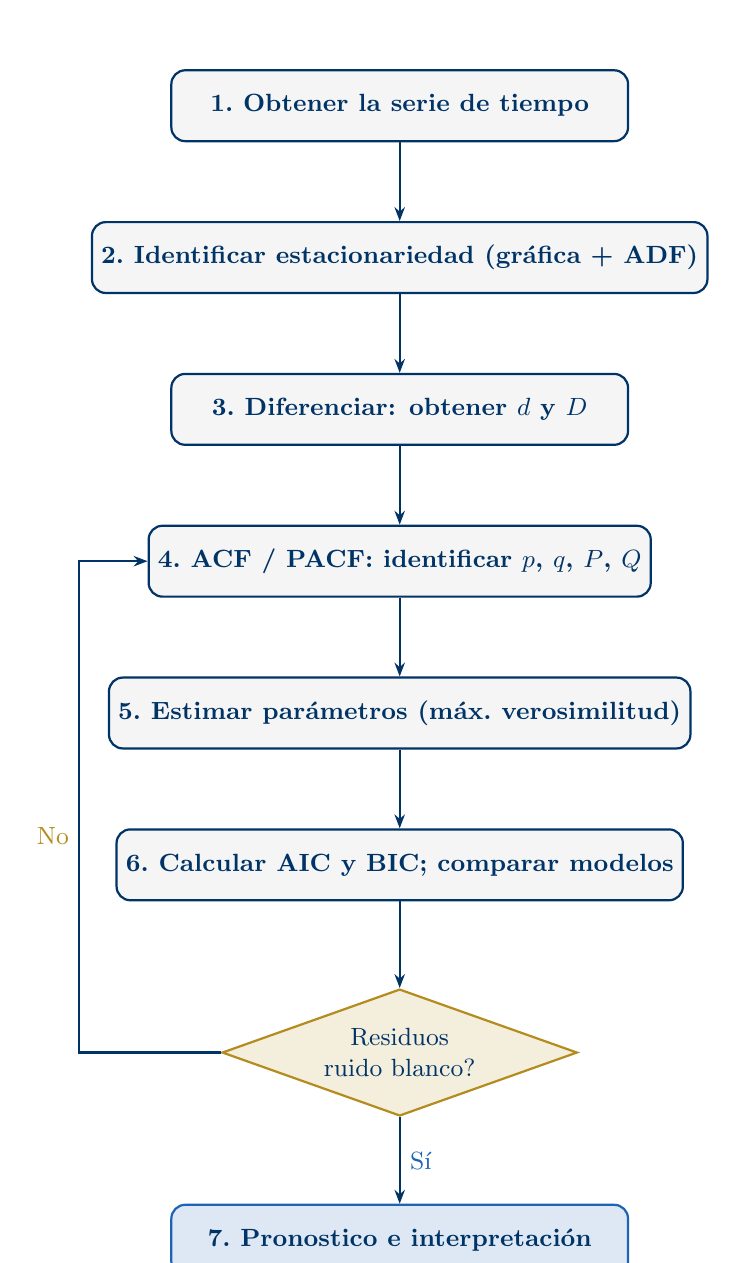
\begin{tikzpicture}[
      node distance=1cm,
      block/.style={draw=upnavy, fill=lightgray, rounded corners=5pt,
                    minimum width=5.8cm, minimum height=0.9cm,
                    align=center, font=\small\bfseries, text=upnavy, thick},
      decision/.style={draw=upgold, fill=upgold!15, diamond,
                       minimum width=3cm, minimum height=1.1cm,
                       align=center, font=\small, text=upnavy, thick, aspect=2.8},
      arrow/.style={-{Stealth[length=5pt]}, thick, color=upnavy},
    ]
    \node[block] (a) {1.\ Obtener la serie de tiempo};
    \node[block, below=of a] (b) {2.\ Identificar estacionariedad (gr\'{a}fica + ADF)};
    \node[block, below=of b] (c) {3.\ Diferenciar: obtener $d$ y $D$};
    \node[block, below=of c] (d) {4.\ ACF / PACF: identificar $p$, $q$, $P$, $Q$};
    \node[block, below=of d] (e) {5.\ Estimar par\'{a}metros (m\'{a}x.\ verosimilitud)};
    \node[block, below=of e] (f) {6.\ Calcular AIC y BIC; comparar modelos};
    \node[decision, below=1.1cm of f] (g) {Residuos\\ruido blanco?};
    \node[block, below=1.1cm of g,
          fill=accentblue!15, draw=accentblue] (h) {7.\ Pronostico e interpretaci\'{o}n};

    \draw[arrow] (a) -- (b); \draw[arrow] (b) -- (c);
    \draw[arrow] (c) -- (d); \draw[arrow] (d) -- (e);
    \draw[arrow] (e) -- (f); \draw[arrow] (f) -- (g);
    \draw[arrow] (g) -- node[right,font=\small,color=accentblue]{S\'i} (h);
    \draw[arrow] (g.west) -- +(-1.8,0)
      |- node[left,font=\small,color=upgold,pos=0.22]{No} (d.west);
  \end{tikzpicture}
  \caption{Metodolog\'{i}a iterativa de Box-Jenkins para construcci\'{o}n de modelos
    ARIMA/SARIMA.}
  \label{fig:boxjenkins}
\end{figure}

% ═══════════════════════════════════════════════════════════════════════════
\section{Conclusiones}
% ═══════════════════════════════════════════════════════════════════════════

\begin{enumerate}[label=\textbf{\arabic*.}]
  \item \textbf{Estacionariedad:} el log-precio del S\&P~500 es no estacionario
    en nivel pero estacionario en primera diferencia ($d=1$), confirmado por la
    prueba ADF y los correlogramas.

  \item \textbf{Identificaci\'{o}n:} la ACF de la primera diferencia muestra corte
    en el rezago 1 ($\Rightarrow q\leq 1$); la PACF muestra corte en el rezago 1
    ($\Rightarrow p\leq 1$). Esto conduce a modelos ARIMA con \'{o}rdenes bajos,
    consistente con la hip\'{o}tesis de mercados eficientes.

  \item \textbf{Selecci\'{o}n:} los criterios AIC y BIC coinciden en seleccionar el
    modelo ARIMA$(1,1,0)$ como el m\'{a}s parsimonioso para los retornos del
    S\&P~500. Agregar par\'{a}metros adicionales no mejora el ajuste.

  \item \textbf{Estacionalidad:} el modelo SARIMA$(1,1,1)(1,1,1)_{12}$ captura
    patrones mensuales como el efecto enero y el efecto septiembre, relevantes
    en estrat\'{e}gias de inversi\'{o}n estacional.

  \item \textbf{Diagn\'{o}stico:} en todos los modelos, los residuos no presentan
    autocorrelaci\'{o}n significativa (Ljung-Box $p > 0.05$) y se distribuyen
    aproximadamente normal, validando las especificaciones.

  \item \textbf{Limitaci\'{o}n principal:} los modelos ARIMA/SARIMA son lineales y
    no capturan heterocedasticidad condicional (efectos ARCH/GARCH) presente en
    los retornos financieros. Para modelar la volatilidad se recomienda extender
    con modelos GARCH.
\end{enumerate}

\vspace{1cm}
\hrule
\vspace{0.4cm}
{\small\textit{Informe elaborado para la materia de Series de Tiempo, Finanzas Cuantitativas,
Universidad Panamericana. Serie de datos: S\&P~500 (2018--2023).
Regina Flores Ch\'{a}vez --- Abril 2026.}}

\end{document}
